\documentclass[12pt, a4paper]{article}
\usepackage{graphicx}

\begin{document}

\begin{center}
	\huge{Physikklausur November 2020}
\end{center}

\section{Planck}
\subsection{Wie ist die Energie eines Photons definiert?}
$E=h*\nu$\\
$E=mc^2$\\
$c=\lambda*f=\lambda*\nu$

\subsection{Planck gilt als "Erfinder" der Quantenmechanik}
\subsubsection{Was war das Bedeutenste an seinen Experimenten?}
Energie wird in Quanten übertragen.
\subsubsection{In welchem Jahr ($\pm$ 5 Jahre) fand die Veröffentlichung der Ergebnisse statt?}
1900

\subsection{Wie groß ist die Ruhemasse eines Photons?}
Ein ruhendes Photon hat keine Masse.

\subsection{Wie hoch ist die Frequenz eines roten Photons der Wellenlänge $630nm$?}
Gegeben: $\lambda=630nm$\\
Gesucht: $\nu$\\\\
$\nu=\frac{c}{\lambda}=\frac{3*10^8\frac{m}{s}}{630nm}=4,76*10^{14}\frac{1}{s}$

\newpage

\section{Hülle-Kern}
Ein Lichtblitz, der monochromatisch bei der Wellenlänge von $530nm$ emittiert, hat eine Energie von $1,3MJ$.

\subsection{Welcher Farbe entspricht die o.a. angegebene Wellenlänge}
grün

\subsection{Was heißt eigentlich monochromatisch?}
Monochromatisch heißt, dass das Licht nur \textit{eine} Wellenlänge hat.

\subsection{Wie viele Photonen werden dabei freigesetzt?}
Gegeben: $\lambda=350nm$; $E_{ges}=1,3MJ$\\
$E=h*\nu=h*\frac{c}{\lambda}$\\
$E_{1Ph}=6,6*10^{-34}Js*\frac{3*10^8\frac{m}{s}}{530*10^{-9}m}=3,74*10^{-18}J$\\
$N=\frac{E_{ges}}{E_{1Ph}}=\frac{1,3*10^6J}{3,74*10^{-18}J}=3,5*10^{24}$

\subsection{Das Licht wird spektralverschoben. Was passiert mit der Anzahl der Photonen bei einer Wellenlänge von $1060nm$? Erkläre plausibel.}
Die Anzahl der Photonen verdoppelt sich, da die Energie pro Photon halbiert wird (verdoppelung der Wellenlänge).

\subsection{Sie kennen das Spektrum eines schwarzen Strahlers. Als ein Beispiel gilt das Sonnenspektrum.}
\subsubsection{Skizzieren Sie das Sonnenspektrum}
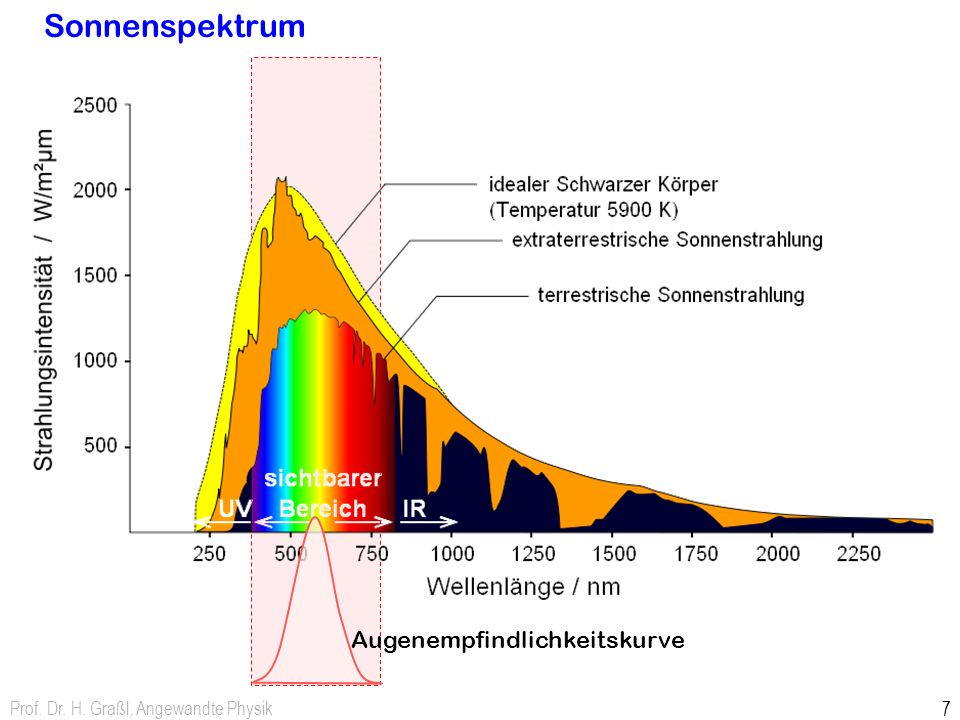
\includegraphics[width=\textwidth]{Sonnenspektrum.jpg}

\subsubsection{Wie berechnen Sie die Anzahl der Photonen in solchen Fällen? Erklären Sie anschaulich.}
Das Integral der Gauss-Kurve korreliert mit der Anzahl der Photonen.

\newpage

\section{Hg-Lampe}
Sie haben das Spektrum einer Hg-Lampe bei den Wellenlängen: $405nm$, $435nm$, $546nm$ und $576nm$ gemessen.

\subsubsection{Wie wird dieses Spektrum bezeichnet?}
Das Spektrum wird als Linienspektrum bezeichnet.

\subsubsection{Berechnen Sie die einzelnen Energien in $eV$.}
$E=h*\nu$\\
$c=\lambda*\nu$\\
$\nu=\frac{c}{\lambda}$\\
$E=h*\frac{c}{\lambda}$\\
$E=6,6*10^{-34}Js*\frac{3*10^8\frac{m}{s}}{305*10^{-9}m}=\frac{4,91*10^{19}J}{1,6*10^{-19}C}=3,06eV$

\subsubsection{Stellen Sie die Ergebnisse maßstabsgetreu als Jablonski-Diagramm dar.}
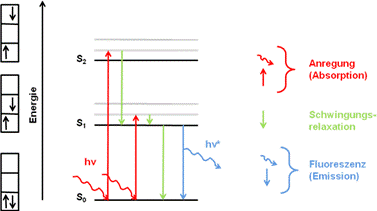
\includegraphics[width=\textwidth]{Jablonski.png}

\subsubsection{Wie wird das o.a. Diagramm noch bezeichnet?}
Termspektrum

\newpage

\section{Photoeffekt}
Monochromatisches Licht der Wellenlänge $546nm$ löst aus einer Metallschicht Fotoelektronen der kinetischen Energie $0,33eV$ aus.
Entscheiden Sie mithilfe der Tabelle, um welches Metall es sich handelt.

\begin{table}[htb]
	\begin{tabular}{|l|l|l|l|l|l|l|}
	\hline
	Metall                & Na   & K    & Cs   & Cu   & Au   & Pt   \\ \hline
	Austrittsarbeit in eV & 2,28 & 2,25 & 1,94 & 4,84 & 4,83 & 5,66 \\ \hline
	\end{tabular}
\end{table}

Gegeben: $\lambda=546nm=546*10^{-9}m$; $E_{kin}=0,33eV$\\
$E_{kin}=h*\frac{c}{\lambda}-E_A$\\
$E_A=\frac{6,63*10^{-34}J}{1,602*10^{-19}\frac{J}{eV}}*\frac{3*10^8\frac{m}{s}}{546*10^{-9}m}-0,33eV$\\
$E_A=1,94eV$\\\\
Es handelt sich also um Cäsium (Cs).

\end{document}
